\section{Architecture logicielle}
Pour ce projet, plusieurs logiciels nous ont été imposés. Cette partie détaille comment ces logiciels seront utilisés pour concevoir l'application.

\subsection{Unity}
\begin{figure}[h]
  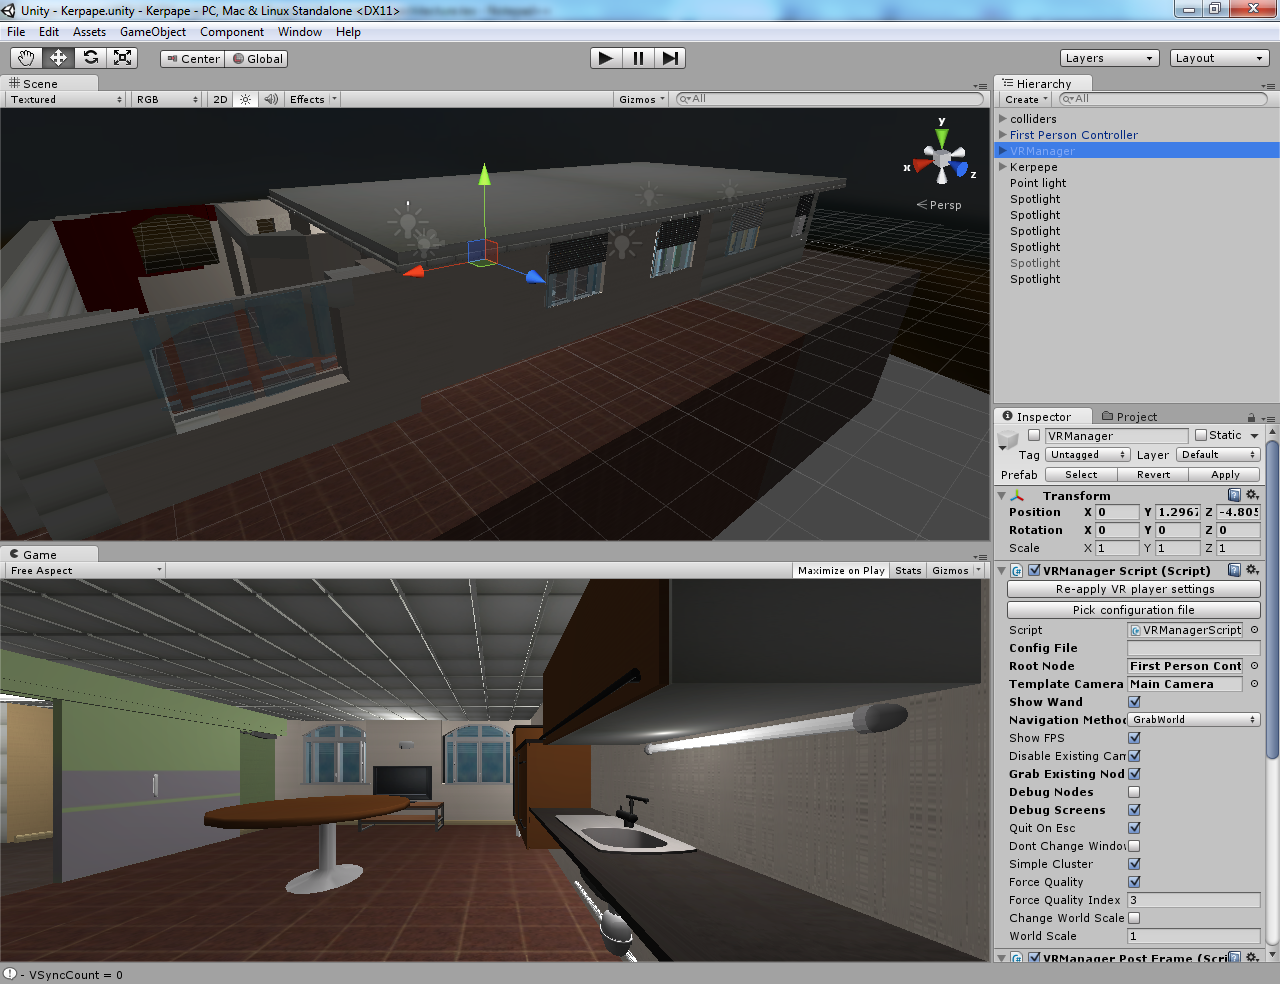
\includegraphics[width=1\textwidth]{4-conception/img/unity_screenshot.png}
  \caption{Capture d'écran : Unity}
  \label{unity}
\end{figure}

Unity (\textsc{figure~\ref{unity}}) est un moteur de jeu et environnement de développement. Bien que Unity donne la possibilité d'insérer des scripts pour gérer les objets plus en profondeur, il permet avant tout de créer une scène 3d. L'utilisateur peut se deplacer à l'interieur, en ayant des interactions avec l'environnement. Unity gère un certain nombre d'éléments, dont :
\begin{itemize}
        \item les colliders : représentent les collisions engendrées par l'objet.
        \item les meshs : correspondent à l'affichage des objets de la scène.
        \item les rigid bodies : soumettent un objet à la physique (notamment pour la gravité).
\end{itemize}


\subsection{MiddleVR}
\begin{figure}[h]
  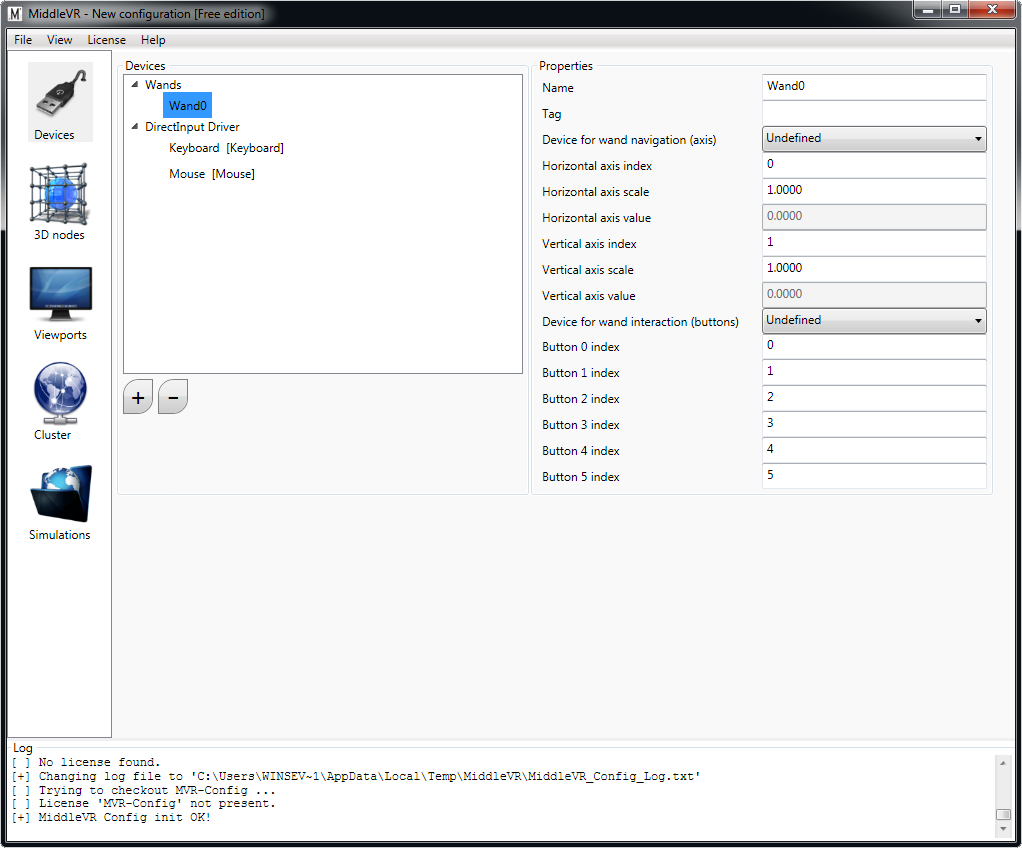
\includegraphics[width=1\textwidth]{4-conception/img/middlevr_screenshot.png}
  \caption{Capture d'écran : MiddleVR}
  \label{middlevr}
\end{figure}
MiddleVR (\textsc{figure~\ref{middlevr}}) est un plugin Unity utilisé pour s'abstraire des périphériques d'entrée/sortie. Il permet de créer un fichier de configuration contenant les informations sur les différents périphériques dont se servira l'application. Pour cela, MiddleVR possède sa propre interface et il n'est pas nécessaire d'écrire du code.
Pour récupérer les valeurs des périphériques dans Unity, on utilise le VRManager, qui sert d'interface entre Unity et MiddleVR.

\subsection{Script C\#}
Unity utilise des scripts en C\# pour réaliser des interactions plus poussées que de simples collisions. Ces scripts nous donnent la possibilité d'allumer ou éteindre une lumière, ou déplacer un objet par exemple. Ils sont l'unique type de code que nous allons produire dans ce projet, il devront donc gérer les différents modes d'apprentissage, ainsi que les scénarios d'utilisation.\newline

Dans Unity, un script est attaché à un objet, il correspond à son comportement. Par exemple, un script attaché à un interrupteur va indiquer ce qu'il se passe lorsque le joueur appuie dessus. Il va commander le changement d'état de l'interrupteur, le changement de lumière (s'il commande la lumière d'une pièce) et éventuellement d'autres éléments selon le mode d'apprentissage.\newline
\begin{figure}[h]
\centering
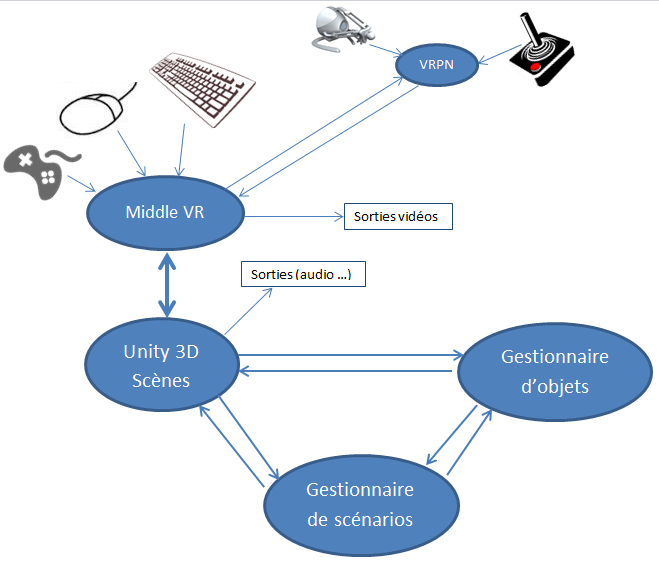
\includegraphics[width=1\textwidth]{4-conception/img/recap.png}
\caption{ Diagramme récapitulatif }
\label{recap}
\end{figure}

Dans la \textsc{figure \ref{recap}}, on peut noter que nous ne communiquons pas avec le VRPN nous-même, MiddleVR s'en charge à notre place. Pour plus d'informations sur le VRPN, voir \url{http://www.middlevr.com/middlevr-for-unity/} ou notre rapport de pré-étude.